\chapter{関連研究と諸概念の整理}
\label{chap:prevresearch}

\section{ユーザビリティ}

英単語としてのusabilityはuse(使う)+able(できる)+ity(こと)から構成されており,「使うのに便利で実用的な」という意味で14世紀から使われていた\cite{oed:usability}\cite{kurosu}.しかし,概念としてのユーザビリティがアカデミアで取り上げられるようになったきっかけはコンピュータの登場と普及だった\cite{kurosu}.コンピュータはトレーニングを受けた専門家が使用するものとして作られたが,一般への普及が図られるなかで使いやすさを検討する必要性が出てきたのだと考えられる.

シャッケルによると彼以前にミラーやベネットがユーザビリティに言及しているが,彼らはユーザビリティを「使いやすさ(ease of use)」とほぼ同義として扱っていた\cite{shackel1991human}\cite{kurosu}.ニールセンは,ユーザビリティを複数の要素の上位概念であるとし,下位概念として学習可能性(Learnabiliity),Efficiency(効率性),Memorability(記憶のしやすさ),Errors(エラー),Satisfication(満足度)を挙げている\cite{nielsen1994}.

国際規格としてユーザビリティが定義されたのはISO9241シリーズ「人間とシステムの相互作用の人間工学(Ergonomics of Human-System Interaction)」であり,ISO9241-11:1998ではユーザビリティを「特定のユーザーが,特定の使用状況において,特定の目標を達成するために,製品を有効,効率的かつ満足に使用できる度合い.(Extent to which a product can be used by specified usersto achieve specified goals witheffectiveness, efficiency and satisfaction in a specified context of use.)」と定義している.この定義はISOの関係者やベヴァンらが普及活動に力を入れた結果標準としての地位を獲得するにいたった\cite{kurosu}.この定義は現在でも一般の技術者に浸透していると考えられる.しかし黒須は,客観的に計測可能な有効性や効率性と主観的なものである満足性を同列に扱うことについて疑問を呈しており,有効かつ効率的であれば満足性が上がるため満足性はより上位の概念であると主張している\cite{kurosu}.

ISO/IEC9126-1:2001やISO/IEC25010:2011 SQuaRE(System and Software Quality Requirements and Evaluation)では体系化が進められており,ユーザビリティが品質モデルの一部に組み込まれた形となっている.SQuaREでは,図\ref{fig:square}のように品質モデルが製品品質モデルと利用時の品質モデルに分けられており,ユーザビリティは製品品質の下位概念に位置づけられている.そして,有効性,効率性,満足性は利用時の品質の中に置かれている.

\begin{figure}[htbp]
  \begin{minipage}{\hsize}
    \begin{center}
       \fbox{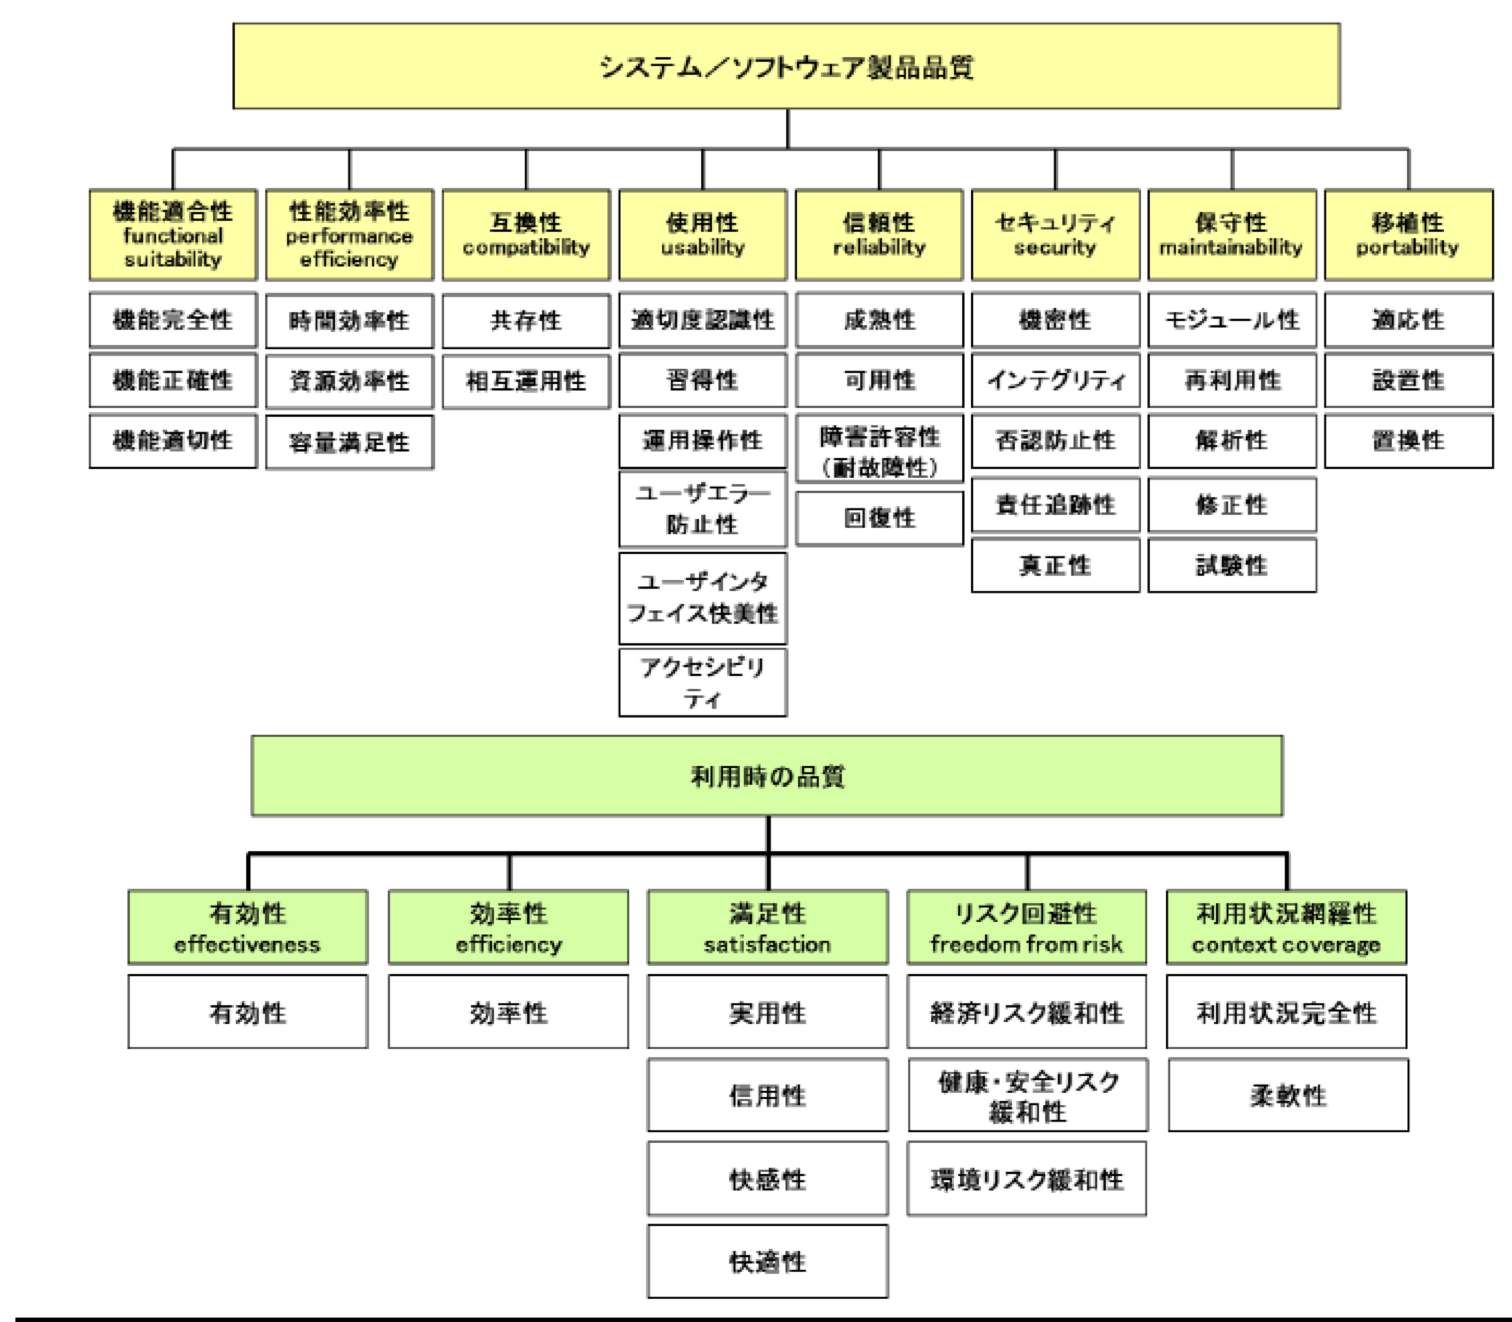
\includegraphics[width=100mm]{square.png}}
    \end{center}
    \caption{SQuaREを基にしたJIS X 25010:2013の品質モデル 画像入れ直すこと}
    \label{fig:square}
  \end{minipage}
\end{figure}

SQuaREの改訂では,設計上の品質である製品品質とユーザが使用した際のユーザにとっての品質である利用時の品質とに分けた点が重要である.人間の思い通り予想通りに動いてくれるシステムを設計しようとする人間中心設計\cite{kurosu2013}の考え方の普及などにより,設計時にユーザの存在をこれまで以上に重要視する動きの中でユーザの利用時に特に注目する必要が出てきたと考えられる.この考え方は後述のUXの概念に関わっており,一方でユーザビリティはユーザに目を向けたものではなく製品設計レベルの概念だということになる.

本研究では,ユーザがシステム利用時にどのような生理的反応を見せるかということに注目しており,SQuaREの定義でいうところの利用時の品質やその下位概念の満足性を測定することを目指しているといえる.第\ref{chap:introduction}章では,ニールセンのヒューリスティック評価はユーザや利用シーンの多様性を考慮しておらず不十分であると述べた.確かにニールセン自身が定義したユーザビリティには満足度が含まれていたためにユーザによってユーザビリティが異なることが考えられた.しかしSQuaREの定義では,ユーザビリティは実ユーザの存在から離れ特定ユーザ・特定の使用状況・特定の目的において満たされていればよく,ニールセンのヒューリスティック評価が有効になると考えられる.一方,本研究で扱うユーザテストでは,ユーザに目が向けられており,SQuaREの定義におけるユーザビリティという概念は当てはめることができない.そこで,SQuaREの利用時の品質などの概念を拡張した概念であるUXについて検討する.なお,本論文ではユーザビリティという用語は基本的に使用せず,使用する場合は「使いやすさ」という一般的な意味でのみ使用する.

\section{UX}

UX白書では \cite{uxwhitepaper}.

\subsection{時間相}

\section{満足性}

\section{UXメトリクス}

ユーザテストでは,パフォーマンスメトリクスや自己申告メトリクス,行動・生理メトリクスを組み合わせて評価することが必要であると前に述べた.パフォーマンスメトリクスでは全ての部分を評価することはできないため,問題がありそうな部分や変更を加えようとする一部分のみを切り出して測定することになる.しかし,この計画立案についてもコストが高くなるため小規模な開発では実施が難しい.



\section{指尖容積脈波}

\section{問題の所在}

\subsection{生理メトリクスの測定手法}
%生理メトリクス関連

\subsection{UXの時間変化の可視化}
%時系列変化関連

\subsection{指尖容積脈波のUX評価への応用}
%指尖容積脈波関連
%まだUXへの応用が少ない
%時系列にしたときの研究が無い